\chapter{Background}\label{ch:background}

\begin{remark}{Outline}
In this chapter, we introduce supervised learning along with fundamental
concepts on which this work builds upon. In Section~\ref{sec:learning-from-data},
we first describe the learning tasks of classification and regression
and then define the notion of model. In Sections~\ref{sec:performance-evaluation}
and \ref{sec:model-selection}, we then proceed with a discussion on
how to evaluate and select the model produced by a learning algorithm. Finally,
we conclude in Section~\ref{sec:classes-of-algorithms} with a brief overview of
some of the main methods in supervised learning.
\end{remark}

\section{Learning from data}
\label{sec:learning-from-data}

In the examples introduced in Chapter~\ref{ch:introduction}, the objective
which is sought is to find a systematic way of predicting a phenomenon given a
set of measurements. In machine learning terms, this goal is formulated as the
{\it supervised learning} task of infering from collected data a model that
predicts the value of an output variable based on the observed values of input
variables. As such, finding an appropriate model is based on the assumption
that the output variable does not take its value at random and that there
exists a relation between the inputs and the output. In medicine for instance,
the goal is to find a decision rule (i.e., a model) from a set of past cases
(i.e., the collected data) for predicting the condition of an incoming patient
(i.e., the output value) given a set of measurements such as age, sex, blood
pressure or history (i.e., the input values).

To give a more precise formulation, let us arrange the set of measurements on a
case in a pre-assigned order, i.e., take the input values to be $x_1, x_2, ...,
x_p$, where $x_j \in {\cal X}_j$ (for $j = 1, ..., p$) corresponds to the value
of the input variable $X_j$. Together, the input values $(x_1, x_2, ..., x_p)$
form a $p$-dimensional input vector $\mathbf{x}$ taking its values in ${\cal
X}_1 \times ... \times {\cal X}_p = {\cal X}$, where ${\cal X}$ is defined as
the input space. Similarly, let us define as $y \in {\cal Y}$ the value of the
output variable $Y$, where ${\cal Y}$ is defined as the output
space\footnote{Unless stated otherwise, supervised learning is reduced to the
prediction of a \textit{single} output variable. More generally however, this
framework can be defined as the prediction of one or several output variables.}.
By definition, both the input and the output spaces are assumed to respectively
contain all possible input vectors and all possible output values. Note that
input variables are sometimes known as {\it features}, input vectors as {\it
objects}, {\it examples} or {\it samples} and the output variable as {\it
target}.

Among variables that define the problem, we distinguish between two general
types. The former correspond to quantitative variables whose values are integer
or real numbers, such as age or blood pressure. The latter correspond to
qualitative variables whose values are symbolic, such as gender or condition.
Formally, we define them as follows:

\begin{definition}
A variable $X_j$ is \emph{numerical} or \emph{ordered} if ${\cal X}_j$ is a
totally ordered set.
\end{definition}

\begin{definition}
A variable $X_j$ is \emph{categorical} if ${\cal X}_j$ is a finite set of values,
without any natural order.
\end{definition}

In a typical supervised learning task, past observations are summarized by a
dataset called {\it learning set}. It consists in a set of observed input
vectors together with their actual output value and formally defined as
follows:

\begin{definition}
A \emph{learning set} ${\cal L}$ is a set of $N$
pairs of input vectors and output values $(\mathbf{x}_1, y_1), ...,
(\mathbf{x}_N, y_N)$, where $\mathbf{x}_i \in {\cal X}$ and $y_i \in {\cal Y}$.
\end{definition}

Equivalently, a set of $p$-input vectors $\mathbf{x}_i$ (for $i=1, ..., N$) can
be denoted by a $N\times p$ matrix $\mathbf{X}$, whose rows $i=1, ..., N$
correspond to input vectors $\mathbf{x}_i$ and columns $j=1, ..., p$ to input
variables $X_j$. Similarly, the corresponding output values can be written as a
vector $\mathbf{y}=(y_1, ..., y_N)$.

\begin{remark}{Data representation}
For optimal implementations of machine learning algorithms, data needs to
represented using structures which allows for high-performance numerical
computation. In this work, code snippets are described under  that assumption
that data is represented using a data structure similar to a NumPy
array~\citep{vanderwalt:2011}.

A NumPy array is basically a multidimensional uniform collection of values, all
of the same type and organized in a given shape. For instance, a matrix
$\mathbf{X}$ can be represented as a 2-dimensional NumPy array of shape $N
\times p$ that contains numbers (e.g., floating point values or integers). This
structure allows for random access in constant time, vectorized high-level
operations and efficient memory usage.

Additionally, using a data representation which is close to the matrix
formulation, like NumPy arrays, makes it possible to write implementations that
are close to their original textbook formulation, thereby making them easier to
understand and maintain. \end{remark}

In this framework, the supervised learning task can be stated as learning a
function $\varphi: {\cal X} \mapsto {\cal Y}$ from a learning set ${\cal
L}=(\mathbf{X}, \mathbf{y})$. In particular, the goal of the learning task is
to find a model such that its predictions $\varphi(\mathbf{x})$, also denoted
by the variable $\hat{Y}$, are as good as possible. If $Y$ is a categorical
variable then the learning task is a classification problem. If $Y$ is
numerical variable, then learning task is a regression problem. Without loss of
generality, the resulting models can be defined as
follows:

\begin{definition}
A \emph{classifier} or \emph{classification rule} is a function $\varphi: {\cal X}
\mapsto {\cal Y}$, where ${\cal Y}$ is a finite set of classes (or labels) denoted $\{0, 1, ..., J-1\}$.
\end{definition}

\begin{definition}
A \emph{regressor} is a function $\varphi: {\cal X} \mapsto {\cal Y}$, where ${\cal Y}=\mathbb{R}$.
\end{definition}

\begin{remark}{Estimator interface}
We follow in this work the API conventions proposed by~\citet{buitinck:2013}.
In particular, learning algorithms are described as \textit{estimator} objects implementing the
following interface:

\begin{itemize}
\item[-] Hyper-parameters of an algorithm are all passed to the constructor of the
estimator. The constructor does not see any actual data. All it does
is to attach hyper-parameters values as public attributes to the estimator object.
\item[-] Learning is performed in a \texttt{fit} method. This method is called with
a learning set (e.g., supplied as two arrays \texttt{X\_train} and \texttt{y\_train}). Its
task is to run a learning algorithm and to determine model-specific parameters
from the data. The \texttt{fit} method always returns the estimator object
it was called on, which now serves as a model and can be used to make predictions.
\item[-] Predictions are performed through a \texttt{predict} method, taking
as input an array \texttt{X\_test} and producing as output the predictions for
\texttt{X\_test} based on the learned parameters. In the case of classification,
this method returns labels from ${\cal Y} = \{0, 1, ..., J-1\}$. In the case of regression,
it returns numerical values from ${\cal Y} = \mathbb{R}$.
\end{itemize}

With this API, a typical supervised learning task is performed as follows:

\vskip0.3cm
\begin{pythoncode}
# Instantiate and set hyper-parameters
clf = DecisionTreeClassifier(max_depth=5)
# Learn a model from data
clf.fit(X_train, y_train)
# Make predictions on new data
y_hat = clf.predict(X_test)
\end{pythoncode}
\end{remark}


\section{Performance evaluation}
\label{sec:performance-evaluation}

In the statistical sense, input and output variables $X_1, ..., X_p$ and $Y$
are \textit{random variables} taking jointly their values from ${\cal X}
\times {\cal Y}$ with respect to the joint probability distribution $P(X, Y)$,
where $X$ denotes the random vector $(X_1, ..., X_p)$. That is,
$P(X=\mathbf{x}, Y=y)$ is the probability of drawing the couple $(\mathbf{x},
y)$ at random from ${\cal X} \times {\cal Y}$.

Accordingly, using an algorithm ${\cal A}$ for learning a model $\varphi$ whose
predictions are as good as possible can be stated as finding a model $\varphi$
which minimizes its expected prediction error, defined as follows:

\begin{definition}
The \emph{expected prediction error}, also known as \emph{generalization
error} or \emph{test error}, of the model $\varphi$ is\footnote{$\mathbb{E}_X \{f(X)\}$ denotes the expected value of $f(x)$
(for $x \in {\cal X}$) with respect to the probability distribution of the
random variable $X$. It is defined as $$\mathbb{E}_X \{f(X)\} = \sum_{x \in {\cal
X}} P(X=x) f(x).$$}
\begin{equation}\label{eqn:generalization-error}
Err_{{\cal L}}(\varphi) = \mathbb{E}_{X, Y}\{ L(Y, \varphi(X)) | {\cal L} \},
\end{equation}
where ${\cal L}$ is the learning set used to build $\varphi$ and $L$ is a loss
function measuring the discrepancy between its two
arguments~\citep{geurts:2002}.
\end{definition}

Equation~\ref{eqn:generalization-error} basically measures the prediction error of $\varphi$ over all
possible couples $(\mathbf{x}, y)\in {\cal X}\times{\cal Y}$, including the
observed couples from the learning set ${\cal L}$ but also all the
\textit{unseen} ones from ${\cal X}\times{\cal Y} \setminus {\cal L}$. Indeed,
the goal is not in fact to make the very-most accurate predictions over the
subset ${\cal L}$ of known data, but rather to learn a model which is correct
and reliable on all possible data.

For classification, the most common loss function is the \textit{zero-one} loss
function\footnote{$1(\text{\textit{condition}})$ denotes the unit function. It
is defined as
$$1(\text{\textit{condition}}) =
\begin{cases}
1 & \text{if \textit{condition} is true}\\
0 & \text{if \textit{condition} is false}
\end{cases}.
$$} $L(Y, \varphi(X)) = 1(Y \neq \varphi(X))$, where all
misclassifications are equally penalized. In this case, the generalization
error of $\varphi$ becomes the probability of misclassification of the model:
\begin{equation}
Err_{\cal L}(\varphi) = \mathbb{E}_{X, Y}\{ 1(Y \neq \varphi(X)) | {\cal L} \} = P(Y \neq \varphi(X)|{\cal L})
\end{equation}

Similarly, for regression, the most used loss function is the \textit{squared
error} loss $L(Y, \varphi(X)) = (Y - \varphi(X))^2$, where large differences
between the true values and the predicted values are penalized more heavily
than small ones. With this loss, the generalization error of the model becomes:
\begin{equation}
Err_{\cal L}(\varphi) = \mathbb{E}_{X, Y}\{ (Y - \varphi(X))^2 | {\cal L} \}
\end{equation}

\subsection{Estimating $Err_{\cal L}(\varphi)$}
\label{sec:estimating-generalization-error}

In practice, the probability distribution $P(X, Y)$ is usually unknown, making
the direct evaluation of $Err_{\cal L}(\varphi)$ infeasible. Equivalently, it
is often not possible to draw additional data, thereby making infeasible the
empirical estimation of $Err_{\cal L}(\varphi)$ on a (virtually infinite) set
${\cal L}'$ drawn independently from ${\cal L}$. In most problems, ${\cal L}$
constitutes the only data available, on which both the model needs to be
learned and its generalization error estimated. As reviewed and described on
multiple occasions by several
authors~\citep{toussaint:1974,stone:1978,breiman:1984,kohavi:1995,nadeau:2003,hastie:2005,arlot:2010},
the generalization error in Equation~\ref{eqn:generalization-error} can however
be estimated in several ways.

To make notations clearer, let us first define $\overline{E}(\varphi^\prime, {\cal
L}^\prime)$ as the average prediction error of the model $\varphi^\prime$ over the set
${\cal L}^\prime$ (possibly different from the learning set used to produce
$\varphi^\prime$), that is:
\begin{equation}
\overline{E}(\varphi^\prime, {\cal L}^\prime) = \frac{1}{N^\prime} \sum_{(\mathbf{x_i}, y_i) \in {\cal L}^\prime} L(y_i, \varphi^\prime(\mathbf{x_i}))
\end{equation}
where $N^\prime$ is the size of the set ${\cal L}^\prime$.

The first and simplest estimate of the generalization error is the
\textit{resubstitution estimate} or \textit{training sample estimate}. It
consists in empirically estimating $Err_{\cal L}(\varphi)$ on the same data as
the learning set ${\cal L}$ used to build $\varphi$, that is:
\begin{equation}\label{eqn:training-error}
\widehat{Err}_{\cal L}^\text{train}(\varphi) = \overline{E}(\varphi, {\cal L})
\end{equation}
In general, the resubstitution error is a poor estimate of $Err_{\cal
L}(\varphi)$. In particular, since most machine learning algorithms aim at
precisely minimizing Equation~\ref{eqn:training-error} (either directly or
indirectly), it typically results in an overly optimistic estimate of the
generalization error -- which accounts for all couples $(\mathbf{x}, y)$, i.e.,
not only those from ${\cal L}$.

The second approach is the \textit{test sample estimate}. It consists in
dividing the learning set ${\cal L}$ into two disjoint sets ${\cal
L}_\text{train}$ and ${\cal L}_\text{test}$, called \textit{training set} and
\textit{test set}, and then to use each part respectively for learning a model
and estimating its generalization error. The test sample estimate of the
generalization error of the model $\varphi$ that would be obtained from ${\cal
L}$ is then given as the average prediction error over ${\cal L}_\text{test}$
of the model $\varphi^\prime$ built on ${\cal L}_\text{train}$:
\begin{equation}\label{eqn:test-error}
\widehat{Err}_{\cal L}^\text{test}(\varphi) = \overline{E}(\varphi^\prime, {\cal L}_\text{test})
\end{equation}
As a rule-of-thumb,
${\cal L}_\text{train}$ is usually taken as $70\%$ of the samples in
${\cal L}$ and ${\cal L}_\text{test}$ as the remaining $30\%$, though
theoretical work~\citep{guyon:1997} suggests to progressively reduce the size of test set as
the size of ${\cal L}$ increases. In any case, care must taken when splitting ${\cal
L}$ into two subsets, so that samples from ${\cal L}_\text{train}$ can be
considered independent from those in ${\cal L}_\text{test}$ and drawn from the
same distribution. This is however usually guaranteed by drawing ${\cal
L}_\text{train}$ and ${\cal L}_\text{test}$ simply at random from ${\cal L}$.
While being an unbiased estimate of $Err_{\cal L}(\varphi)$, the test sample
estimate has the drawback that it reduces the
effective sample size on which the model $\varphi^\prime$ is learned. If ${\cal L}$ is large,
then this is usually not an issue, but if ${\cal L}$ only contains a few dozens
of samples, then this strategy might not correctly approximate the true
generalization error of the model that would have been learned on the entire learning set.

When ${\cal L}$ is small, the \textit{$K$-fold cross-validation estimate} is
usually preferred over the test sample estimate. It consists in randomly
dividing the learning set ${\cal L}$ into $K$ disjoint subsets, denoted  ${\cal
L}_1, ..., {\cal L}_K$, and then to estimate the generalization error $Err_{\cal
L}(\varphi)$ as the average prediction error over the folds ${\cal L}_k$ of the
models $\varphi_k$  learned on the remaining data ${\cal L}\setminus{\cal
L}_k$:
\begin{equation}\label{eqn:cv-error}
\widehat{Err}_{\cal L}^{CV}(\varphi) = \frac{1}{K} \sum_{k=1}^K  \overline{E}(\varphi_k, {\cal L}_k)
\end{equation}
The assumption behind this approach is that since each model $\varphi_k$ is
built using almost all ${\cal L}$, they should all be close to the model
$\varphi$ learned on the entire set ${\cal L}$. As a result the unbiased
estimates $\overline{E}(\varphi_k, {\cal L}_k)$ should also all be close to
$Err_{\cal L}(\varphi)$. While more computationally intensive, the $K$-fold
cross-validation estimate has the advantage that every couple $(\mathbf{x}, y)
\in {\cal L}$ is used for estimating the generalization error of $\varphi$. In
a typical setting, $K$ is usually fixed to $10$, a value often yielding stable
and reliable estimates~\citep{kohavi:1995}.

\begin{remark}{Expected generalization error}
As we have shown, our goal is to estimate the generalization error $Err_{\cal
L}(\varphi)$ conditional on the learning set ${\cal L}$. A related quantity
is the \textit{expected} generalization error
\begin{equation}\label{eqn:expected-generalization-error}
Err = \mathbb{E}_{\cal L} \{ Err_{\cal L}(\varphi) \},
\end{equation}
averaging over everything which is random, including the randomness in the
learning set ${\cal L}$ used to produce $\varphi$. As discussed by
\citet{hastie:2005}, this quantity is close, yet different from $Err_{\cal
L}(\varphi)$. In particular, the authors point out that most estimates, including $K$-fold
cross-validation, effectively estimate
Equation~\ref{eqn:expected-generalization-error} rather than
Equation~\ref{eqn:generalization-error}.
\end{remark}

\subsection{Bayes model and residual error}
\label{sec:bayes-model}

When the probability distribution $P(X, Y)$ is known, the best possible model,
i.e., the model $\varphi_B$ which minimizes the generalization error of
Equation~\ref{eqn:generalization-error}, can be derived analytically and
independently of any learning set ${\cal L}$.

By conditioning on $X$, the generalization error of this model can be rewritten as:
\begin{equation}\label{eqn:generalization-error-conditionned}
\mathbb{E}_{X, Y}\{ L(Y, \varphi_B(X)) \} = \mathbb{E}_{X}\{ \mathbb{E}_{Y|X} \{ L(Y, \varphi_B(X)) \} \}
\end{equation}
In this latter form, the model which minimizes
Equation~\ref{eqn:generalization-error-conditionned} is a model which
minimizes the inner expectation pointwise, that is:
\begin{equation}
\varphi_B(\mathbf{x}) = \argmin_{y \in {\cal Y}} \mathbb{E}_{Y|X=\mathbf{x}} \{ L(Y, y) \}
\end{equation}
In the literature, $\varphi_B$ is known as the \textit{Bayes model} and its
generalization error $Err(\varphi_B)$ as the \textit{residual error}. It represents the minimal
error that any supervised learning algorithm can possibly attain, that is
the irreducible error purely due to random deviations in the data.

\begin{definition}
A model $\varphi_B$ is a \emph{Bayes model} if, for any model $\varphi$ built from any
learning set ${\cal L}$, $Err(\varphi_B) \leq Err_{\cal L}(\varphi)$.
\end{definition}

In classification, when $L$ is the zero-one loss, the Bayes model is:
\begin{align}
\varphi_B(\mathbf{x}) &= \argmin_{y \in {\cal Y}} \mathbb{E}_{Y|X=\mathbf{x}} \{ 1(Y, y) \} \nonumber \\
                      &= \argmin_{y \in {\cal Y}} P(Y \neq y|X=\mathbf{x}) \nonumber \\
                      &= \argmax_{y \in {\cal Y}} P(Y = y|X=\mathbf{x}) \label{eqn:bayes-model-classification}
\end{align}
Put otherwise, the best possible classifier
consists in systematically predicting the most likely class $y \in \{0, 1, ..., J-1\}$
given $X=\mathbf{x}$.

Similarly, for regression with the square error loss, we have:
\begin{align}
\varphi_B(\mathbf{x}) &= \argmin_{y \in {\cal Y}} \mathbb{E}_{Y|X=\mathbf{x}} \{ (Y - y)^2 \} \nonumber \\
                      &= \mathbb{E}_{Y|X=\mathbf{x}} \{ Y \} \label{eqn:bayes-model-regression}
\end{align}
In other words, the best possible regressor consists in systematically predicting
the average value of $Y$ at $X=\mathbf{x}$.

For practical problems, $P(X, Y)$ is unknown and the Bayes model cannot be
derived analytically. In this context, the effectiveness of a model $\varphi$
may be difficult to evaluate since (estimates of) $Err_{\cal L}(\varphi)$ may
not be very indicative of the goodness of $\varphi$ if the lowest attainable
error $Err(\varphi_B)$ is unknown. On simulated data however, where the
distribution is known, deriving $\varphi_B$ and $Err(\varphi_B)$ is feasible.
This is beneficial as $Err(\varphi_B)$ can now be used for comparing the
test set error of $\varphi$ and thereby evaluate the
actual effectiveness of $\varphi$ with respect the best model one can
possibly build.

From a theoretical point of view, the concepts of Bayes model and residual
error are also useful to study the learning capabilities of an algorithm. In
particular, as ${\cal L}$ gets arbitrarily large, a fundamental question is to
know whether it is possible to produce a model $\varphi$ which is
\textit{consistent}, that is such that its generalization error gets
arbitrarily close to the lowest possible generalization error $Err(\varphi_B)$.
Formally, consistency is defined as follows~\citep{devroye:1996}:

\begin{definition}
A learning algorithm ${\cal A}$ is said to be \emph{consistent} for a certain distribution
$P(X, Y)$ if $\mathbf{E}_{\cal L} \{ Err_{\cal L}(\varphi) \} \to Err(\varphi_B)$
as the size $N$ of the learning set ${\cal L}$ used to build $\varphi$ using ${\cal A}$ tends
to infinity.
\end{definition}

\begin{definition}
A learning algorithm ${\cal A}$ is said to be \emph{strongly consistent} for a certain distribution
$P(X, Y)$ if $Err_{\cal L}(\varphi) \to Err(\varphi_B)$ almost surely
as the size $N$ of the learning set ${\cal L}$ used to build $\varphi$ using ${\cal A}$ tends
to infinity.
\end{definition}

Note that the definition of consistency depends on the distribution $P(X, Y)$.
In general, a model $\varphi$ can be proven to be consistent for some
classes of distributions, but not for others. If consistency can be proven
for any distribution $P(X, Y)$, then $\varphi$ is said to be \textit{universally}
(strongly) consistent.


\section{Model selection}
\label{sec:model-selection}

From the previous discussion in Section~\ref{sec:bayes-model}, it appears that
to solve the supervised learning problem it would be sufficient to estimate
$P(Y|X)$ from the learning sample ${\cal L}$ and then to define a model
accordingly using either Equation~\ref{eqn:bayes-model-classification} or
Equation~\ref{eqn:bayes-model-regression}. Unfortunately, this approach is
infeasible in practice because it requires ${\cal L}$ to grow exponentially
with the number $p$ of input variables in order to compute accurate estimates of
$P(Y|X)$~\citep{geurts:2002}.

\subsection{Selecting the (approximately) best model}

To make supervised learning work in high-dimensional input spaces with learning
sets of moderate sizes, simplifying or restrictive assumptions must be made on
the structure of the best model $\varphi_B$. More specifically, a supervised
learning algorithm assumes that $\varphi_B$ -- or at least a good enough approximation
-- lives in a family ${\cal H}$ of candidate models, also known as
\textit{hypotheses} in statistical learning theory, of restricted structure. In
this setting, the \textit{model selection} problem is then defined as finding
the best model among ${\cal H}$ on the basis of the learning set ${\cal L}$.

\begin{remark}{Approximation error}
Depending on restrictions made on the structure of the problem, the
Bayes model usually does not belong to ${\cal H}$, but there may be models
$\varphi \in {\cal H}$ that are sufficiently close to it. In particular, the
\textit{approximation error}~\citep{bottou:2011} measures how closely the
models in ${\cal H}$ can approximate the optimal model $\varphi_B$:
\begin{equation}
Err({\cal H}) = \min_{\varphi \in {\cal H}} \{ Err(\varphi) \} - Err(\varphi_B)
\end{equation}
where $Err(\varphi)$ is the generalization error of $\varphi$ (independently
of any learning set ${\cal L})$.
\end{remark}

To be more specific, let $\theta$ be the vector of hyper-parameters values
controlling the execution of a learning algorithm ${\cal A}$. The application
of ${\cal A}$ with parameters $\theta$ on the learning set ${\cal L}$ is a
deterministic\footnote{If ${\cal A}$ makes use of a pseudo-random generator to
mimic a stochastic process, then we assume that the corresponding random seed is
part of $\theta$.} process yielding a model ${\cal A}(\theta, {\cal L}) =
\varphi \in {\cal H}$. As such, our goal is to find the vector of hyper-parameters values
yielding to the best model possibly learnable in ${\cal H}$ from ${\cal L}$:
\begin{equation}
\theta^* = \argmin_{\theta} Err_{\cal L}({\cal A}(\theta, {\cal L}))
\end{equation}
Again, this problem cannot (usually) be solved exactly in practice since
it requires the true generalization error of a model to be computable. However
approximations $\widehat{\theta}^*$ can be obtained in several ways.

When ${\cal L}$ is large, the easiest way to find $\widehat{\theta}^*$ is to
use test sample estimates (as defined by Equation~\ref{eqn:test-error}) to
guide the search of the hyper-parameter values, that is:
\begin{align}
\widehat{\theta}^* &= \argmin_{\theta} \widehat{Err}^\text{test}_{\cal L}({\cal A}(\theta, {\cal L})) \\
                   &= \argmin_{\theta} \overline{E}({\cal A}(\theta, {\cal L}_\text{train}), {\cal L}_\text{test})
\end{align}
In practice, solving this later equation is also a difficult task but
approximations can be obtained in several ways, e.g., using either manual
tuning of $\theta$, exhaustive exploration of the parameter space using grid
search, or dedicated optimization procedures (e.g., using random
search~\citep{bergstra:2012}). Similarly, when ${\cal L}$ is scarse, the same
procedure can be carried out in the exact same way but using $K$-fold
cross-validation estimates (as defined by Equation~\ref{eqn:cv-error}) instead of test sample
estimates. In any case, once $\widehat{\theta}^*$ is identified, the learning
algorithm is run once again on the entire learning set ${\cal L}$, finally
yielding the approximately optimal model ${\cal A}(\widehat{\theta}^*, {\cal
L})$.

When optimizing $\theta$, special care must taken so that the resulting model
is neither too simple nor too complex. In the former case, the model is indeed
said to \textit{underfit} the data, i.e., to be not flexible enough the capture
the structure between $X$ and $Y$. In the later case, the model is said to
\textit{overfit} the data, i.e., to be too flexible and to capture illusory
structures that are specific to the learning set.

\begin{figure}
    \centering
    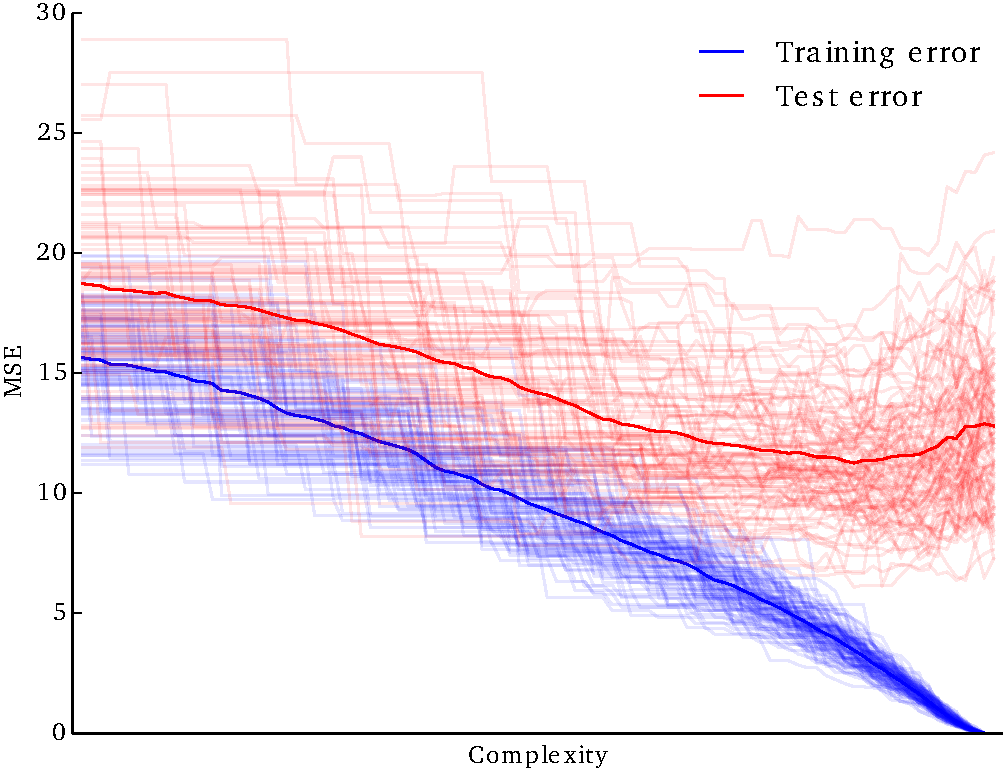
\includegraphics[scale=0.5]{figures/ch2_train_test_error.pdf}
    \caption{Training and test error with respect to the complexity
             of a model. The light blue curves show the training error over
             ${\cal L}_\text{train}$ while the light red curves show the test
             error estimated over ${\cal L}_\text{test}$ for $100$ pairs of training
             and test sets ${\cal L}_\text{train}$ and ${\cal L}_\text{test}$
             drawn at random from a known distribution. The thick blue curve
             is the average training error while the thick red curve is the
             average test error. (Figure inspired from \citep{hastie:2005}.) }
    \label{fig:train-test-error}
\end{figure}

As Figure~\ref{fig:train-test-error}
illustrates, this phenonemon can be observed by examining the
respective training and test estimates of the model with respect to its
complexity. When the model is too simple, both the training and test estimates
are large because of underfitting. As complexity increases, the model gets more
accurate and both the training and test estimates decrease. However, when the
model becomes too complex, specific trends from the training set get captured,
reducing the corresponding training estimates down to $0$, as if the model were
perfect. At the same time, the test estimates become worse because the
structure learned from the training set is actually too speficic and does not
generalize. The model is overfitting. The best parameter value $\theta$ is
therefore the one making the appropriate trade-off and producing a model which
neither too simple nor to complex.

\subsection{Selecting and evaluating simultaneously}
On real applications, and in particular when reporting results, it usually
happens that one wants to do both model selection and model assessment. That
is, having chosen a final model ${\cal A}(\widehat{\theta}^*, {\cal L})$, one
wants to also estimate its generalization error.

A naive assessment of the generalization error of the selected model might be
to simply use the test sample estimate $\smash{\widehat{Err}^\text{test}_{\cal
L}({\cal A}(\widehat{\theta}^*, {\cal L}))}$ (i.e., $\overline{E}({\cal
A}(\widehat{\theta}^*, {\cal L}_\text{train}), {\cal L}_\text{test})$) that was
minimized during model selection. The issue with this estimate is that the
learned model is not independent from ${\cal L}_\text{test}$ since its repeated
construction was precisely guided by the minimization of the prediction error
over ${\cal L}_\text{test}$. As a result, the minimized test sample error is in
fact a biased, optimistic, estimate of the true generalization error, sometimes
leading substantial understimations. For the same reasons, using the $K$-fold
cross-validation estimate does not provide a better estimate since model
selection was similarly guided by the minimization of this quantity.

To guarantee an unbiased estimate, the test set on which the generalization
error is evaluated should ideally be kept out of the entire model selection
procedure and only be used once the final model is selected.
Algorithm~\ref{algo:train-valid-test} details such a protocol. Similarly,
per-fold estimates of the generalization error should be kept out of the model
selection procedure, for example using nested cross-validation within each
fold, as explicited in Algorithm~\ref{algo:cv}.

\begin{algorithm}\label{algo:train-valid-test}
Train-Valid-Test set protocol for both model selection and evaluation.

\begin{enumerate}
\item Divide the learning set ${\cal L}$ into three parts
      ${\cal L}_\text{train}$, ${\cal L}_\text{valid}$ and ${\cal L}_\text{test}$;
\item Perform model selection on ${\cal L}_\text{train} \cup {\cal L}_\text{valid}$
      using test sample estimates, i.e., find:
      \begin{align}
      \widehat{\theta}^* &= \argmin_{\theta} \widehat{Err}_{{\cal L}_\text{train} \cup {\cal L}_\text{valid}}^\text{test}({\cal A}(\theta, {\cal L}_\text{train} \cup {\cal L}_\text{valid})) \\
                         &= \argmin_{\theta} \overline{E}({\cal A}(\theta, {\cal L}_\text{train}), {\cal L}_\text{valid});
      \end{align}
\item Evaluate the (unbiased) generalization error of the final model as
      \begin{equation}
      \overline{E}({\cal A}(\widehat{\theta}^*, {\cal L}_\text{train} \cup {\cal L}_\text{valid}), {\cal L}_\text{test});
      \end{equation}
\item Learn the final model ${\cal A}(\widehat{\theta}^*, {\cal L})$ on the entire learning set.
\end{enumerate}
\end{algorithm}

\begin{algorithm}\label{algo:cv}
Nested $K$-fold cross-validation protocol for both model selection and evaluation.

\begin{enumerate}
\item Divide the learning set ${\cal L}$ into $K$ folds ${\cal L}_1, ..., {\cal L}_K$;
\item For each fold $k=1, ..., K$:
    \begin{enumerate}
        \item Divide ${\cal L}\setminus{\cal L}_k = {\cal L}^{-k}$ into $K$ folds ${\cal L}_1^{-k}, ..., {\cal L}_K^{-k}$;
        \item Perform model selection on the subset ${\cal L}^{-k}$ using nested $K$-fold estimates, i.e., find:
        \begin{align}
            \widehat{\theta}_k^* &= \argmin_{\theta} \widehat{Err}_{{\cal L}^{-k}}^{CV}({\cal A}(\theta, {\cal L}^{-k}))\\
                                 &= \argmin_{\theta} \frac{1}{K} \sum_{l=1}^K \overline{E}({\cal A}(\theta, {\cal L}^{-k} \setminus {\cal L}_l^{-k}), {\cal L}_l^{-k});
        \end{align}
        \item Evaluate the generalization error of the selected sub-model as
        \begin{equation}
            \overline{E}({\cal A}(\widehat{\theta}^*_k, {\cal L}\setminus{\cal L}_k), {\cal L}_k);
        \end{equation}
    \end{enumerate}
\item Evaluate the (unbiased) generalization error of the selected model as the average generalization estimate of the sub-models selected over the folds:
\begin{equation}
\frac{1}{K} \sum_{k=1}^K \overline{E}({\cal A}(\widehat{\theta}^*_k, {\cal L}\setminus{\cal L}_k), {\cal L}_k);
\end{equation}
\item Perform model selection on the entire learning set ${\cal L}$ using $K$-fold cross-validation estimates, i.e., find:
\begin{align}
    \widehat{\theta}^* &= \argmin_{\theta} \widehat{Err}_{\cal L}^{CV}({\cal A}(\theta, {\cal L}))\\
                       &= \argmin_{\theta} \frac{1}{K} \sum_{k=1}^K \overline{E}({\cal A}(\theta, {\cal L} \setminus {\cal L}_k), {\cal L}_k);
\end{align}
\item Learn the final model ${\cal A}(\widehat{\theta}^*, {\cal L})$ on the entire learning set.
\end{enumerate}
\end{algorithm}


\section{Classes of learning algorithms}
\label{sec:classes-of-algorithms}

% As introduced in Section~\ref{sec:model-selection}, classes of  learning
% algorithms can be defined in terms of the space ${\cal H}$ of hypotheses  they
% are built upon.
Before proceeding in the next chapters, and for the rest of
this work, to an in-depth analysis of the class of tree-based methods,  we
briefly review in this section some of the other learning algorithms that have
matured in the field, including linear methods, neural networks and nearest
neighbor methods.

\subsection{Linear methods}

One of the oldest class of supervised learning algorithms is the class of
\textit{linear methods} from the field of statistics. In these methods, the central
assumption made on ${\cal H}$ is that the output variable $Y$ can be described
as a linear combination of the input variables $X_1, ..., X_p$, or at least
that the linear model is a reasonable approximation. For regression, ${\cal H}$
includes all models $\varphi$ of the form:
\begin{equation}
\varphi(\mathbf{x}) = w_0 + \sum_{j=1}^p x_j w_j
\end{equation}
For binary classification (i.e., when ${\cal Y}=\{0, 1\}$),  ${\cal H}$ includes all
models $\varphi$ of the form:
\begin{equation}
\varphi(\mathbf{x}) = \begin{cases}
1 & \text{if } w_0 + \sum_{j=1}^p x_j w_j > 0\\
0 & \text{otherwise}
\end{cases}
\end{equation}

Linear methods come in many flavours but mostly differ from each other in the
way they estimate the coefficients $w_j$, usually using some specific
optimization procedure to minimize a specific criterion. Among all of them, the
most famous is the method of \textit{least squares}. It consists in finding the
$w_j$ coefficients that minimize the resubstitution estimate
(Equation~\ref{eqn:training-error}) using the squared error loss.

Despite an apparent simplicity, linear methods often provide reliable
predictions and an interpretable description of how the input variables affect
the output. Contrary to their name, linear methods can also be used to model
non-linear relations between $X$ and $Y$, for example by applying these methods
on (non-linear) transformations of the input variables. For more details on
(generalized) linear methods, see the reviews of \citet{maccullagh:1989},
\citet{hastie:2005}, \citet{bishop:2006} or \citet{duda:2012}.

\subsection{Neural networks}

The family of \textit{neural networks} methods finds its origins in attempts to
identify mathematical representations of information processing in biological
systems. While this objective is still far from being reached, (artificial)
neural networks have nonetheless proven all their worth from a statistical point of
view, and have actually grown into one of the most effective methods in machine
learning.

A neural network is usually made of several units, also known as \textit{neurons}, of the form
\begin{equation}
h_j(\mathbf{x}) = \sigma(w_j + \sum_{i=1}^n w_{ij} x_i),
\end{equation}
where $\sigma$ is a non-linear activation function, such as the sign function,
the sigmoid function or the softmax activation. In most cases, these units are
structured into successive layers, where the outputs of a layer are directed
through weighted connections, also known as \textit{synapses}, to the inputs of
the next layer. As an example, Figure~\ref{fig:mlp} illustrates a three layered
neural network. The first layer is the input layer, which transmits the input
values $\mathbf{x} = (x_1, ..., x_p)$ to the second layer. The second layer is
made of activation units $h_j$, taking as inputs the weighted values of the
input layer and producing non-linear transformations as outputs. The third
layer is made of a single activation unit, taking as inputs the weighted
outputs of the second layer and producing the predicted value $\hat{y}$.
Assuming that this structure is fixed and that all units from the network make
use of the same activation function $\sigma$, the hypothesis space ${\cal H}$
therefore includes all models $\varphi$ of the form
\begin{equation}
\varphi(\mathbf{x}) = \sigma(w_5 + \sum_{j=1}^4 w_{j5} \sigma(w_j + \sum_{i=1}^p w_{ij} x_i)).
\end{equation}

\begin{figure}
    \centering
    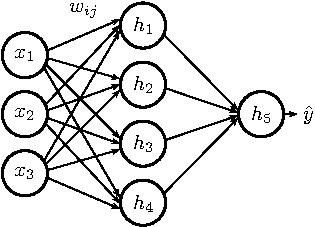
\includegraphics[scale=1.0]{figures/ch2_mlp.pdf}
    \caption{An artificial neural network.}
    \label{fig:mlp}
\end{figure}

As for linear methods, learning a neural network  amounts to estimate the
weights $w_{ij}$ that minimize some specific loss function, using some specific
optimization procedure. Among all of them, the most famous is the
\textit{backpropagation algorithm}.

Recent advances on neural networks, now themed as \textit{deep learning}, have
recently shown the capability of these models to autonomously learn high-level
and very effective representations of data. On various difficult tasks, such as
image classification or speech recognition, neural networks have indeed
achieved outstanding performance, outperforming both human operators and
state-of-the-art methods. From a theoretical point of view however, little is
still known about what makes them truly work. In particular, picking the
appropriate combination of number of units, layers and types of activation
functions remains a delicate task, which unfortunately makes (deep) neural
networks still difficult to use for non-experts. Reviews on recent developments
include the works of \citet{hinton:2007}, \citet{arel:2010} or \citet{bengio:2013}.

\subsection{Nearest neighbor methods}

\textit{Nearest neighbor methods} belong to a class of non-parametric algorithms
known as \textit{prototype methods}~\citep{hastie:2005}. They distinguish from
other learning algorithms in the sense that they are memory-based and require
no model to be fit.

The principle behind nearest neighbor methods is to find a number of
training samples closest in distance to the new sample, and then infer from
these the value of the output variable. For regression, the $k$-nearest
neighbor algorithm~\citep{fix:1951} averages the output values from the $k$
closest training samples, that is:
\begin{equation}
\varphi(\mathbf{x}) = \frac{1}{k} \sum_{(\mathbf{x_i}, y_i) \in NN(\mathbf{x}, {\cal L}, k)} y_i,
\end{equation}
where $NN(\mathbf{x}, {\cal L}, k)$ denotes the $k$ nearest neighbors of ${\mathbf{x}}$ in ${\cal L}$.
For classification, the procedure is the same except that the predicted
output value is computed as the majority class among the $k$ nearest neigbors:
\begin{equation}
\varphi(\mathbf{x}) = \argmax_{c \in {\cal Y}} \sum_{(\mathbf{x_i}, y_i) \in NN(\mathbf{x}, {\cal L}, k)} 1(y_i = c).
\end{equation}
In general, the distance function used to identify the $k$ nearest neighbors
can be any metric, but the standard Euclidean distance is the most common
choice. A notable variant is the
\textit{radius-based neighbor algorithm}, in which the predicted output value
is computed from the training samples within a radius $r$ of the new sample.
In cases where data is not uniformly sampled, this latter algorithm can be
a better choice than the $k$-nearest neighbor method.

Despite their simplicity, nearest neighbor methods usually yield very good
results in practice. In particular, they are are often successful in
classification situations where the decision boundary is very irregular. From a
theoretical point of view, an important result due to \citet{cover:1967} is the
proof of consistency of the method. When the size of ${\cal L}$ tends to
infinity and $k$ is appropriately adjusted to ${\cal L}$, the generalization
error of the model produced by the $k$-nearest neighbor method is shown to
converge towards the generalization error of the Bayes model.
